\chapter{Pre-integrazione}


\section{Studio frontend}
Per creare una chat nei moderni siti web dinamici \'e stato necessario lo studio di un linguaggio che sicuramente ha modernizzato lo sviluppo web cio\'e JavaScript soprattutto per la quantit\'a impressionante di framework sviluppati con questa tecnologia.
\'E un linguaggio interpretato, che ha molto poco a che fare con il quasi omonimo Java, la prima versione venne rilasciata nel 1995 con l'obbiettivo di arricchire le pagine web aggiungendo alcune forme di dinamicit\'a. L'utilizzo in una pagina \'e possibile solo se il browser del client possiede un supporto a interpretare il linguaggio, questa scelta di mantenere la responsabilit\'a a livello client \'e stata fatta per non sovracaricare troppo il server che riliasciava il servizio web relativo.
\iffalse 
<studio di angularjs nel libro (vedi https://github.com/Wabri/UniversityInternship#day-01-020518--55-ore)>
\fi
Le prime fasi di tirocinio le ho concentrate sull'apprendimento dei vari strumenti necessari per comprendere l'architettura della web application formata principalmente da codice HTML con direttive AngularJS e Javascript, tenuti insieme dal MVC (Model View Controller).
Il MVC \'e un pattern architetturale basato su 3 componenti che hanno lo scopo di usare e gestire i dati con scopi differenti: il model deve gestire i dati e fornire metodi per usarli nonch\'e la logica e le regole dell'applicazione, il view ha lo scopo di rappresentare i dati sotto forma di informazione in modo tale da interagire con l'utente che li visualizzer\'a, e infine il controller che attraverso istruzioni fornite dall'utente modifica lo stato degli altri 2 componenti modificando i dati gestiti dal controller o indicando una modalit\'a differente di visualizzazione dei dati al view.
\begin{figure}[H]
 \centering
  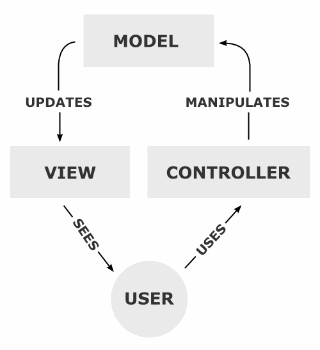
\includegraphics[width=0.3\textwidth]{img/MVC-Process.png}
 \caption{MVC}
 \end{figure}
Questa struttura viene usata principalmente per dividere la logica di business, che \'e la parte di eleborazione dati, con l'interfaccia utente, migliorando quindi l'organizzazione dei processi interni di una application. 
L'utilizzo di questo pattern direttamente sul client ha permesso un cambiamento importante per quanto riguarda le dynamic pages, cio\'e quello di non eseguire un redirect per modificare la pagina ma eseguendo chiamate asincrone al server. 
Con il tempo \'e stato necessario fornire un framework che implementasse queste logiche riducendo i tempi di sviluppo andando a generalizzare tutti quei comportamenti classici del pattern MVC, se si parla di JavaScript senza alcun dubbio il framework pi\'u usato \'e AngularJs.
Questa libreria funziona per mezzo di comandi, definiti direttive, che vengono inserite direttamente nel codice HTML che permettono di eseguire una sorta di comunicazione tra le varie parti del client. Il framework viene caricato all'interno della pagina attraverso l'import definito dal tag <script> in questo modo:
\lstset{ 
  backgroundcolor=\color{white},   % choose the background color; you must add \usepackage{color} or \usepackage{xcolor}; should come as last argument
  basicstyle=\footnotesize,        % the size of the fonts that are used for the code
  breakatwhitespace=false,         % sets if automatic breaks should only happen at whitespace
  breaklines=true,                 % sets automatic line breaking
  captionpos=b,                    % sets the caption-position to bottom
  commentstyle=\color{green},    % comment style
  deletekeywords={...},            % if you want to delete keywords from the given language
  escapeinside={\%*}{*)},          % if you want to add LaTeX within your code
  extendedchars=true,              % lets you use non-ASCII characters; for 8-bits encodings only, does not work with UTF-8
  firstnumber=0,                % start line enumeration with line 1000
  frame=single,	                   % adds a frame around the code
  keepspaces=true,                 % keeps spaces in text, useful for keeping indentation of code (possibly needs columns=flexible)
  keywordstyle=\color{blue},       % keyword style
  language=HTML,                 % the language of the code
  morekeywords={*,...},            % if you want to add more keywords to the set
  numbers=none,                    % where to put the line-numbers; possible values are (none, left, right)
  numbersep=5pt,                   % how far the line-numbers are from the code
  numberstyle=\tiny\color{gray}, % the style that is used for the line-numbers
  rulecolor=\color{black},         % if not set, the frame-color may be changed on line-breaks within not-black text (e.g. comments (green here))
  showspaces=false,                % show spaces everywhere adding particular underscores; it overrides 'showstringspaces'
  showstringspaces=false,          % underline spaces within strings only
  showtabs=false,                  % show tabs within strings adding particular underscores
  stepnumber=2,                    % the step between two line-numbers. If it's 1, each line will be numbered
  stringstyle=\color{mauve},     % string literal style
  tabsize=3,	                   % sets default tabsize to 2 spaces
  title=\lstname                   % show the filename of files included with \lstinputlisting; also try caption instead of title
}
\begin{lstlisting}
<script 
 src="https://ajax.googleapis.com/ajax/libs/angularjs/1.2.19/angular.js">
</script>
\end{lstlisting}
Questo script esegue una lettura dell'intera pagina dove saranno presenti le direttive che dovr\'a eseguire che modificheranno (o no) le sezioni che vogliamo essere dinamiche della pagina.

\section{Creazione della chat stand alone}
Apprese le conoscenze base di questi strumenti ho cominciato con la stesura di una prima versione della chat testuale stand alone in JavaScript. Una chat presuppone la comunicazione tra pi\'u di 2 soggetti, nel mio caso un soggetto \'e rappresentato da l'utente della banca che usa la chat e l'altro il bot, una comunicazione di questo tipo è possibile implementarla usando i sockets.
I sockets sono la soluzione migliore per chat real-time che prevedouno una communicazione bidirezionale tra un client e server, questo prevede quindi che un client mandi un messaggio in chat e il server prende l'incarico di ridirezionare il messaggio al destinatario effettivo. Un socket rimane attivo in ascolto in un canale di comunicazione permettendo lo scambio in input e output di messaggi, in base al tipo di messaggio il socket eseguir\'a una azione specifica che nel caso di una chat \'e stampare o inviare un messaggio. Per fare questo ho usato una libreria JavaScript chiamata socket.io (https://socket.io) che tramite il metodo emit permette di emettere un messaggio in output:
\lstdefinelanguage{JavaScript}{
  keywords={typeof, new, true, false, catch, function, return, null, catch, switch, const, var, if, in, while, do, else, case, break},
  keywordstyle=\color{blue}\bfseries,
  ndkeywords={class, export, boolean, throw, implements, import, this},
  ndkeywordstyle=\color{darkgray}\bfseries,
  identifierstyle=\color{black},
  sensitive=false,
  comment=[l]{//},
  morecomment=[s]{/*}{*/},
  commentstyle=\color{purple}\ttfamily,
  stringstyle=\color{red}\ttfamily,
  morestring=[b]',
  morestring=[b]"
}
\lstset{
   language=JavaScript,
   backgroundcolor=\color{white},
   extendedchars=true,
   basicstyle=\footnotesize\ttfamily,
   showstringspaces=false,
   showspaces=false,
   numbers=left,
   numberstyle=\footnotesize,
   numbersep=9pt,
   tabsize=2,
   breaklines=true,
   showtabs=false,
   captionpos=b
}
\begin{lstlisting}
// inviare un messaggio
socket.emit('text message', text);
\end{lstlisting} 
Una volta che il messaggio viene emesso un altro socket deve ricevere questo messaggio, \'e quindi necessario che il socket del controller sia sempre in ascolto di messaggi e in base al tipo del messaggio esegua una determinata azione:
\begin{lstlisting}
// connessione e gestione del messaggio
const io = require('socket.io')(server);
io.on('connection', function (socket) {
    socket.on('text message', (text) => {
        // gestione del messaggio
    });
});
\end{lstlisting}
Uno dei motivi principali dello sviluppo di un chatbot \'e quello di permettere all'utente di parlare direttamente al bot usando la voce. Per fare questo ho dovuto usare uno strumento che trasformasse la voce catturata dal microfono in un testo, per la precisione in una stringa da poter inviare tramite il socket al server, un tool di questo tipo \'e definito speech recognition, in italiano riconoscimento vocale.
Ho usato una libreria sviluppata da mozilla chiamata proprio SpeechRecognition (https://developer.mozilla.org/en-US/docs/Web/API/SpeechRecognition) una volta impostata la lingua ha permesso di trasformare il parlato dell'utente in una stringa utilizzabile all'interno del client. 
Nel codice HTML ho inserito semplicemente un bottone che una volta attivato il microfono abilita la funzione di speech recognition, una volta che l'utente smette di parlare verr\'a restituita la stringa risultante che verr\'a inviata tramite socket.
\begin{lstlisting}
// Dichiarazione
const SpeechRecognition = window.SpeechRecognition
const recognition = new SpeechRecognition();
// Proprieta'
recognition.lang = 'it-IT';
recognition.interimResults = false;
// event listener click button
document.querySelector('button').addEventListener('click', () => {
    recognition.start();
});
// event listener result recognition
recognition.addEventListener('result', (e) => {
    let last = e.result.length - 1; 
    let text = e.result[last][0].transcript;
    socket.emit('chat message', text);
});
// event listener end recognition
recognition.addEventListener('speechend', () => {
  recognition.stop();
});
\end{lstlisting}
Inviato il messaggio dell'utente all'intelligenza questa genera una risposta che viene stampata nella pagina, per rendere naturale la conversazione ho deciso di dare una voce al bot introducendo il procedimento inverso dello speech to text. Per fare questo ho usato la funzione fornita da mozilla chamata SpeechSynthesisUtterance (https://developer.mozilla.org/en-US/docs/Web/API/SpeechSynthesisUtterance) che mi ha permesso di trasformare un testo in audio dando cos\'i una voce al bot.
\begin{lstlisting}
function synthVoice(text) {
    const synth = window.speechSynthesis;
    const utterance = new SpeechSynthesisUtterance();
    utterance.text = text;
    synth.speak(utterance);
}
// event bot reply
socket.on('bot reply', function (replyText) {
    synthVoice(replyText);
});
\end{lstlisting}
L'ultima cosa da fare per la parte frontend \'e stata una web interface minimale che permettesse di testare il funzionamento del bot, quindi c'era bisogno di: un bottone che attivasse lo speech to text, una casella di testo nel caso in cui non si vuole usare il microfono e 2 zone di testo dove riportare gli ultimi messaggi scambiati.
\begin{figure}[H]
 \centering
  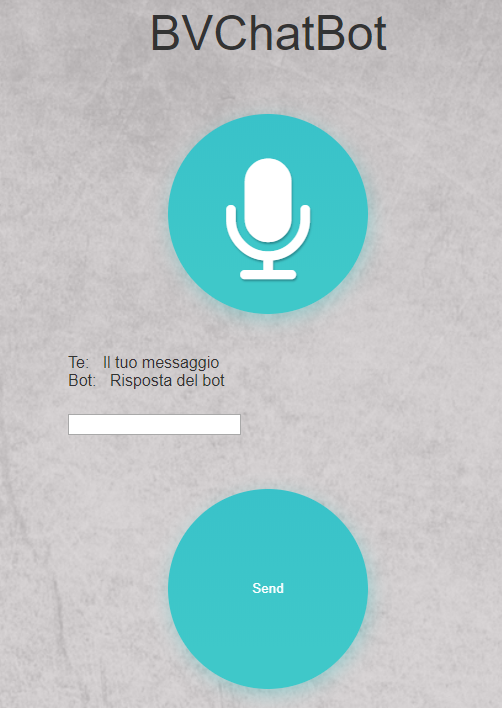
\includegraphics[width=0.4\textwidth]{img/prototype.png}
 \caption{Chat prototype}
\end{figure}

\section{Creazione dell'intelligenza artificiale}
\iffalse
<inserimento della comunicazione tra la chat e dialogflow>
<vari test di funzionamento della comunicazione>
<passaggio da dialogflow a rasa>
<studio di rasa nlu>
https://en.wikipedia.org/wiki/Human_computation
https://en.wikipedia.org/wiki/AI-hard
https://en.wikipedia.org/wiki/Human_computation
https://en.wikipedia.org/wiki/Dialogflow
https://dialogflow.com/
\fi
Per poter compiere una conversazione il bot deve essere creato con dei sistemi di natural language understanding e un'intelligenza artificiale per eseguire azioni necessarie per comprendere e rispondere alle richieste fornite dall'utente.
Il natural language understanding (NLU) \'e una branca dell'intelligenza artificiale che cerca metodi di analizzare un testo per comprendere il significato della frase per permettere di estrarre informazioni importanti, quali l'intento della frase e le caratteristiche principali estraibili dalla frase in input. Problemi di questo tipo sono considerati AI-Hard, chiamati anche AI-Complete, cio\'e non risolvibili con un semplice algoritmo ma \'e necessaria la supervisione dell'uomo che addestra l'intelligenza a risolvere un problema specifico.
Data la complessit\'a di questo compito ho ricercato uno strumento che eseguisse la funzione di NLU e quello che mi \'e sembrato pi\'u vicino alle mie necessit\'a era lo strumento chiamato Dialogflow che forniva tutti gli strumenti necessari per quello che il bot avrebbe dovuto fare.
Dialogflow \'e un tool sviluppato da google per la creazione di conversazioni utente macchina in linguaggio naturale permettendo di sfruttare una tecnologia di questo tipo in qualsiasi contesto necessario, un punto di forza di questo strumento \'e l'interfaccia web molto semplificata per utenti anche alle prime armi.
Per creare un'intelligenza artificiale di questo tipo \'e importante creare un dataset con degli esempi chiari di frasi specificando tutti gli elementi necessari, per il natural language understanding cio\'o di cui si ha bisogno \'e definire per ogni frase di esempio: l'intento e se ci sono delle entit\'a estraibili. 
L'intento \'e il concetto principale che ci permette di indicare l'obbiettivo della frase per distinguere i vari casi che possono presentarsi durante la conversazione con un utente, avere un dataset con una popolazione varia per ogni tipo di intento che si vuole riconoscere \'e importante per permettere una precisione maggiore. 
Le entit\'a sono invece tutti quegli oggetti che all'interno della frase risultano importanti per un uso esterno, per esempio se la richiesta dell'utente \'e il pagamento di 300 euro l'entit\'a che andremo a definire sar\'a 300 che corrisponder\'a al quantitativo di euro che dovremo richiedere di trasferire.  
Il primo dataset che ho creato con Dialogflow era formato da pochi esempi di richieste di pagamento che ho indicato con l'intento chiamato \textbf{payRequest} formato da entit\'a \textbf{receiver}, \textbf{quantity} e \textbf{currency}.
Il motivo della creazione di un dataset ristretto mi ha permesso di avere tempo di integrare questo nuovo strumento con il frontend testando i metodi di conversazione e l'effettivo funzionamento della chat.

\section{Aggiornamento Frontend per la comunicazione con Rasa}

\section{Sistema di pagamento vocale}

\section{Funzionamento e esecuzione}

\iffalse
<creazione di un primo modello di training con vari esempi esterni al progetto>
<processo di apprendimento del funzionamento effettivo di rasa lungo>
<tentativo di utilizzo del modello creato precedentemente, con dialogflow, per la creazione del modello di rasa nlu>
<passaggio di competenze(?) da dialogflow a rasa, eliminando la comunicazione effettiva con google>
<connessione con il server bps e rasa>
<per errore ho lasciato che la chat inviasse ancora i dati di test ai server di dialogflow = rasa>dialogflow>
<tutor universitario consiglia l'uso di typescript => studio di typescript => riscrittura della chat usando typescript>
<typescript migliore lettura del codice e possibilità di creazione di classi e oggetti>
<estrapolazione dei dati utente dal server della banca usando chiamate rest>
<generazione data set dell'intelligenza artificiale>
<necessario un server che eseguisse azioni richieste>
<studiare python per poter creare esempi di rasa core>
<studio di rasa core - server>
<utilizzo di chiamate rest all'interno del chatbot verso rasa core>
<problemi con la messa in opera del server su macchina windows>
<utilizzo del server su rete locale per i test>
<refactor del codice chatbot usando superagent (vedi https://github.com/Wabri/UniversityInternship#day-26-110718--55-ore)>
<iniziato a creare le story per generare un modello efficace di intelligenza>
<Cominciato a generare le prime azioni di risposta in base agli intenti e al contenuto del testo fornito in input>
<Creato l'effettivo bot scritto in python, dove risiedono tutte le azioni che può fare il bot>
<Migliorato il modello di training aggiungendo nuovi esempi di intents e stories>
<problemi con l'autenticazione a 2 fattori per il prototipo, non riesce a estrarre direttamente user e password e devo inserirle manualmente con chiamate post verso il server rasa>
<completamento comunicazione user-rasafrontend-rasabackend-backendspringbanca - vedi https://github.com/Wabri/UniversityInternship/blob/master/README.md#day-36-020818--65-ore>
<creazione delle azioni effettive che deve fare il bot rasa backend>
<il problema del xcsrf token e jsession>
<vedi https://github.com/Wabri/UniversityInternship/blob/master/README.md#day-38-210818--75-ore per maggiori informazioni>
<documentazione prototipo>
\fi